\begin{figure}[H]
    \centering




    \tikzset{every picture/.style={line width=0.75pt}} %set default line width to 0.75pt        

    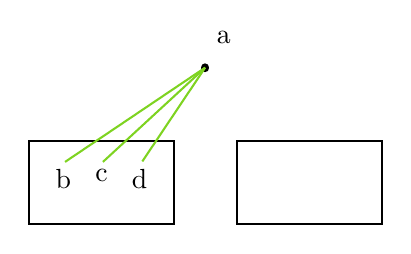
\begin{tikzpicture}[x=0.75pt,y=0.75pt,yscale=-1,xscale=1]
    %uncomment if require: \path (0,300); %set diagram left start at 0, and has height of 300
    
    %Shape: Rectangle [id:dp05929262611884156] 
    \draw   (80,70.25) -- (150,70.25) -- (150,110.25) -- (80,110.25) -- cycle ;
    %Shape: Rectangle [id:dp4641637777411629] 
    \draw   (180.25,70) -- (250.25,70) -- (250.25,110) -- (180.25,110) -- cycle ;
    %Shape: Free Drawing [id:dp486851933115376] 
    \draw  [line width=3] [line join = round][line cap = round] (165,34.93) .. controls (165,34.84) and (165,34.76) .. (165,34.68) ;
    %Straight Lines [id:da7642309413451847] 
    \draw [color={rgb, 255:red, 126; green, 211; blue, 33 }  ,draw opacity=1 ]   (165,34.76) -- (97.5,80.18) ;
    %Straight Lines [id:da4565983768062105] 
    \draw [color={rgb, 255:red, 126; green, 211; blue, 33 }  ,draw opacity=1 ]   (165,34.76) -- (115.75,80.18) ;
    %Straight Lines [id:da3386816838548048] 
    \draw [color={rgb, 255:red, 126; green, 211; blue, 33 }  ,draw opacity=1 ]   (165,34.76) -- (134.75,79.93) ;
    
    
    % Text Node
    \draw (169,16) node [anchor=north west][inner sep=0.75pt]   [align=left] {a};
    % Text Node
    \draw (91.5,82) node [anchor=north west][inner sep=0.75pt]   [align=left] {b};
    % Text Node
    \draw (110.58,82.5) node [anchor=north west][inner sep=0.75pt]   [align=left] {c};
    % Text Node
    \draw (128.25,82) node [anchor=north west][inner sep=0.75pt]   [align=left] {d};
    
    
    \end{tikzpicture}
    
\end{figure}